\documentclass[11pt,letterpaper]{article}

\usepackage{fullpage}
%\usepackage{nips15submit_e,times}
\usepackage{hyperref}
\usepackage{url}
\usepackage{float}
\usepackage{graphicx}
\usepackage{blindtext}
\usepackage{amsmath}
\usepackage{titling}
\usepackage{lipsum}

% preambles 
\title{EECS 545 Project Progress Report: \\
        Tempo-Lite: Drum Beats Generated from Other Instruments}

\author{Congni Shi, Li Ye, Muye Jia, Jerry Cheng\\
        \texttt{\{congni, yeliqd ,muyej, chengjry\}@umich.edu}
}
        

% document body
\begin{document}

% title
\maketitle

% \begin{abstract}
    Comparing to Vision, Audio generation has always been a field that is less studied with deep learning. In ths course project, a lightened version of a temporal music generator MuseGAN \cite{musegan}, Tempo-Lite, is proposed. The Tempo-Lite model takes the existing tracks of musical instruments other than drum and generate complementary drum tracks for the existing tracks. As a milestone of this objective, the group has also provided classification methods and model for the Pianoroll representation of music signals. Although the project is still in progress, the classification models has shown some promising results that can be used in following stages. The group has also finished the Generator and will soon be tested once the Discriminator is finished.  
\end{abstract} %% Jerry

\section{Introduction}
    \label{sec:introduction}
     \begin{par}
    \par \hspace{15pt} Machine learning has been employed extensively in the field of computer vision and image processing, however,it has not been extensively investigated in the music field. For this project, the group aims to use various machine learning models to do music genre classification and music composition. More particularly, the group intends to produce a drum track generator model, which takes the the rest of the song (song tracks without the drum track) and the predicted genre as inputs, then outputs a drum track sequentially based on those inputs.
\end{par}

\begin{par}
    \par \hspace{15pt} Compared to copious deep learning researches in vision, acoustic generative networks are less visited. The group believes that it would be a lucrative field since amateur composers may not be able to compose for all instruments, which means most of them are more familiar with some instruments than the others. In that case, our model, with the ability to generate a music track (drum track) based on tracks from other instruments, can provide important insights for those amateur composers with their music compositions. Moreover, since the aim of the group is to provide a computationally-light training model, it can be easily re-trained towards different musical instruments, even novel ones such as theremin or Kazoo with contemporary styles. 
    
\end{par} %% Congni

\section{Proposed Method}
    \label{sec:proposed}
     \begin{par}
    \begin{figure}[H]
        \centering
        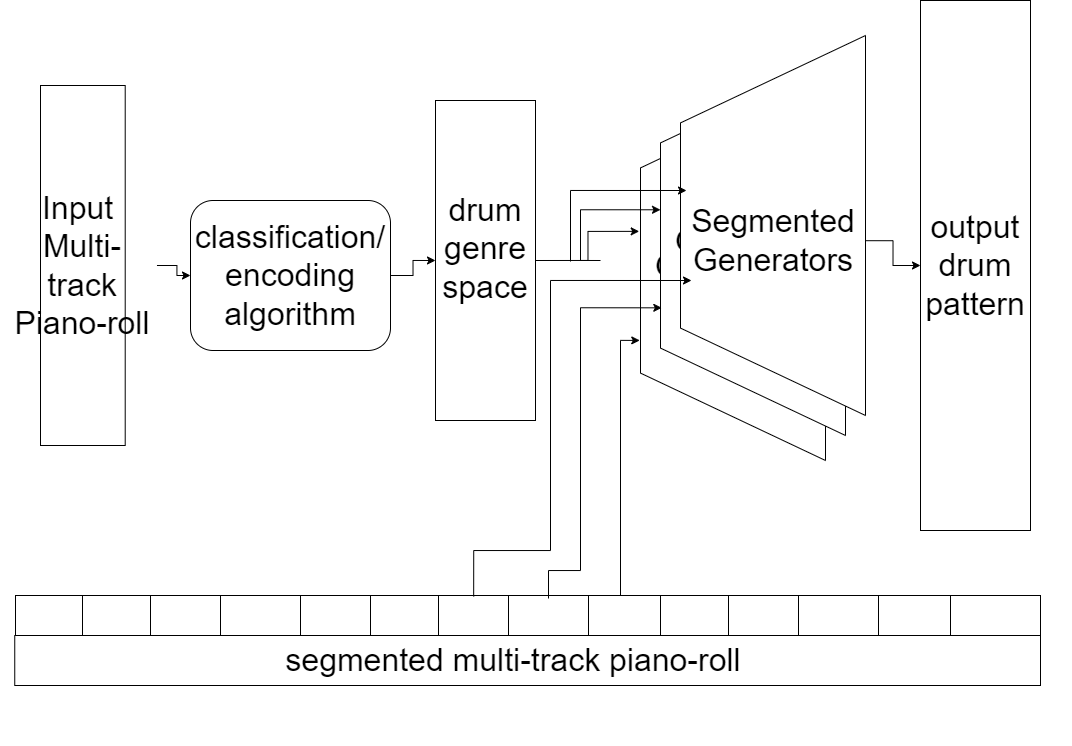
\includegraphics[width=3in]{image/proposal_architecture}
        \caption{General Pipeline the model}
        \label{fig:archie}
    \end{figure}
\end{par}

\begin{par}
    \par \hspace{15pt} Figure 1 shows the general pipeline of the proposed model. The model can be split into 2 parts: classification and generation. The output (before the last layer) of the classifier is fed into the generator as global induction. After that, the generator and the discriminator work together as a Generative Adversarial Network (GAN) to produce the final output.
\end{par} %% Congni

    \subsection{Classification for Global Induction}
        \label{sub:class}
        % \begin{par}

    \begin{figure}[H]
        \centering
        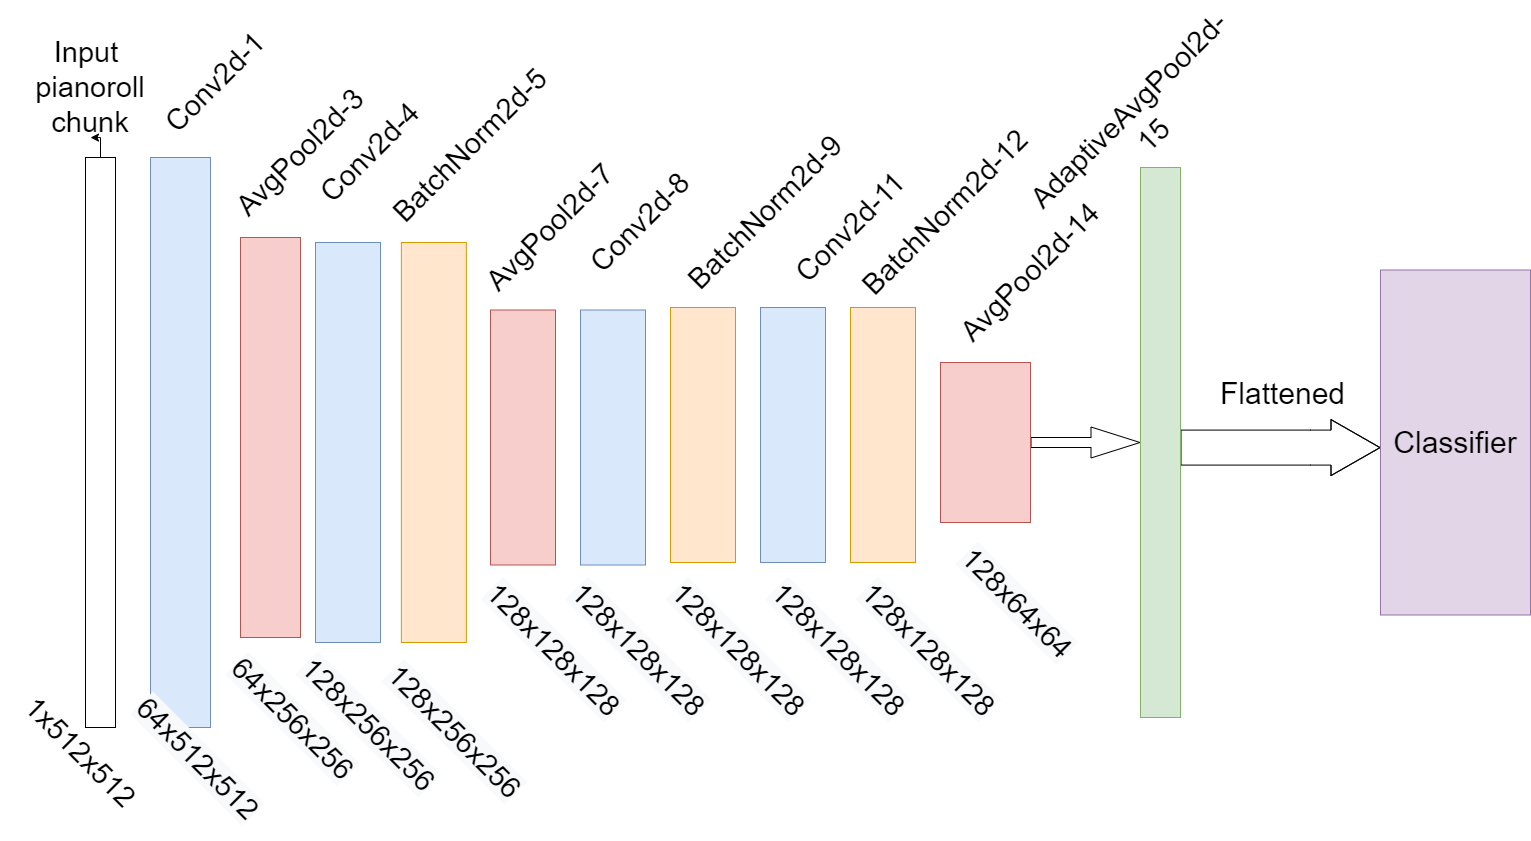
\includegraphics[width=4in]{image/cnn_classifier_feature_architecture}
        \caption{The feature extraction architecture of the CNN classifier}
        \label{fig:cnn_feature}
    \end{figure}

    \par \hspace{15pt} The first classification method the group proposed is a convolutional neural network (CNN) based classifier. The CNN classifier is based on the VGG-16 architecture, featuring convolution layers with small $3 \times 3$ filters. However to adapt the binary nature of the pianoroll, the team decided to replace the max pooling layers into average pooling layers to introduce more structural properties of the data as induction for the model. A more specific architecture will be discussed in the next several paragraphs.

    \par \hspace{15pt} Figure \ref{fig:cnn_feature} shows the feature extraction architecture of the CNN classifier. The feature extraction is done by convolutional layers stride of 2 and padding of $1$. We decided not to pad the input too much to maintain the structure of the binary data. The average pooling layers all have a kernel size of $2$ and stride of $2$ with no padding. The non-linear layer used in the feature extractor was ReLU. 
    
    \begin{figure}[H]
        \centering
        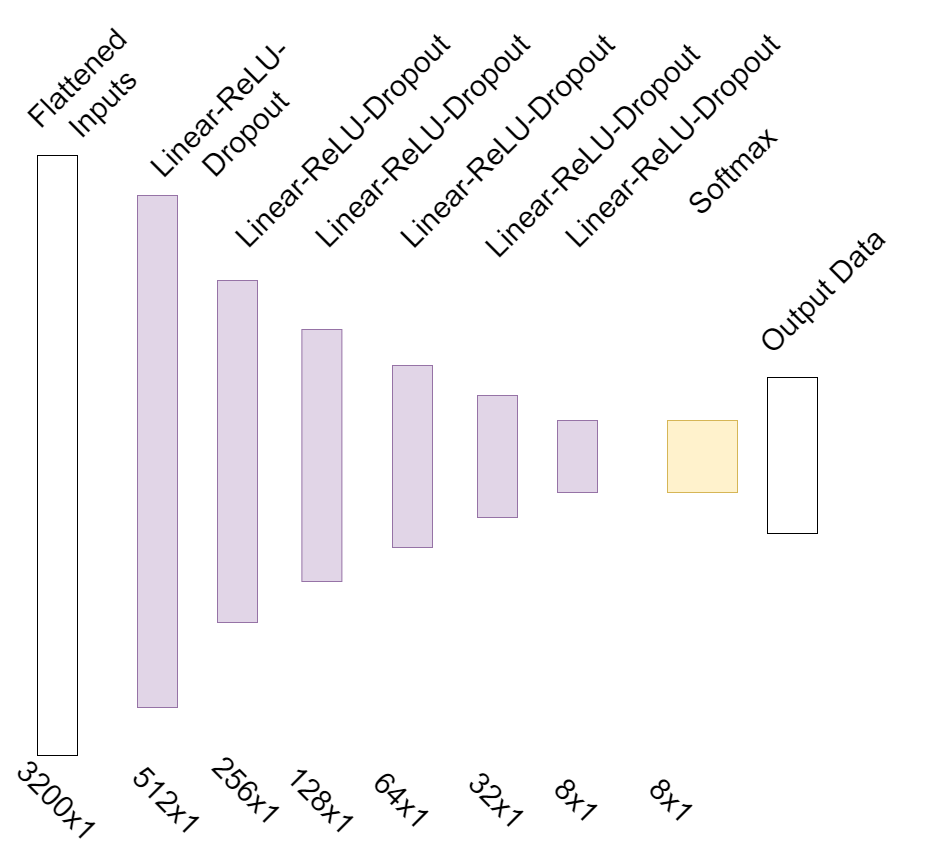
\includegraphics[width=4in]{image/cnn_classifier_architecture}
        \caption{Linear Classifier of the CNN classifier}
        \label{fig:cnn_class}
    \end{figure}
    
    \par \hspace{15pt} The output of the convolutional layers are pooled into a single vector. The output of the pooling layer is fed into a linear classifier, which is shown in Figure \ref{fig:cnn_class}. Dropout layers in the linear classifier shares a probability of $0.3$. Since we believe that can be used to prevent overfitting due to the small training set. In the end, the output of the linear-ReLU-Dropout layers was fed into a softmax layer for classification.

\end{par} %% Jerry
        % \begin{par}
    \par \hspace{15pt} Subspace learning is another method that the group proposed for genre classification. First, for the pre-processing of the data, 512 rows with the highest 0-norm (with the most notes played) are selected to represent the entire song. After that, For each genre, we construct a training set, and then use Singular Value Decomposition (SVD) to obtain an orthonormal basis for each genre space. Some related training can be seen in \cite{pca}. After having learned the genre subspaces, classification can be done by comparing the projections of one particular test data onto the orthogonal complement of the genre subspaces. If a song is the closest to a particular genre subspace among all the genre subspaces, then this song is classified as that particular genre. 
\end{par}


 %% Congni
        % \begin{par}
    \par \hspace{15pt} Although not implemented yet, the group would also like to try the classification task with the Perceiver \cite{perceiver} , which is a sparse attention transformer model with general perception. This classifier would be adapted from a group member's EECS-542, Advance Computer Vision course project, which is expected to be done in the next few weeks.  
\end{par} %% Jerry

    \subsection{Generator}
        % \begin{par}
    \par The team proposes to use Generator Network to generate pieces of music. Each input of the Generator has 
    multiple sub-components, and each sub-component of the Generator has three channels-first channel is a randomly 
    extracted song segment, the second channel contains the genre vector of the song, and lastly the third channel contains the positional
    encoding of the notes in the song segment. All the song segments in each individual input are extracted from the same song, meaning
    they share the same genre vector, which, as the name indicates, tells the Generator the genre of the song that's being fed in; in order
    to preserve a richer spatial connectivity, the team decides to add positional encoding for each time-step. 
    
    Adding positional encoding enriches the information fed into the Generator. It enables the Generator to take into account the spatial 
    connectivity of the beats. Similar to processing a string of words, the ordering of the words is probably the most important information in
    determining the meaning of the sentence-so is the ordering of the notes in a song-the team is hoping that the positional encoding can provide
    this ordering information to the Generator. The advantage of this adopted positional encoding lies in: 1) its ability to provide unique coding
    for the note at each time-step. 2) its ability to generalize to input of arbitrary length. 3) the encoding does not explode as the input length
    increases. 

\end{par} %% Muye
    
    \subsection{Discriminator}
        % \begin{par}
      \par To evaluate the similarity between the generated vector and 
      the vector in the data sample -- i.e. to check whether the model-generated drum beats 
      fit with provided music notes-we propose (as an initial proposition) to use Euclidean distance for 
      measuring the similarity between two vectors. Specifically, the group is considering L1 or L2 
      distance metric. The error calculation works as the following: 
      \begin{equation}
          \emph{J}(w) = \frac{1}{N} \sum_{i=1}^{N} (\norm{G(\mathbf{z})-x^{(i)}})^2
      \end{equation}
      where $G(\mathbf{z})$ represents generated drum beat vector, and $x^{(i)}$
      represents the data sample in training data set. The discriminator will denote the generated drum 
      beat as adequate as long as the above error is lower than a threshold value.
  
  \end{par} %% Muye
        % \input{proposed_traditional} %% Jerry
        % \input{proposed_wasserstein} %% Congni


\section{Related Work}
    \label{sec:related}
    % \begin{par}
    \par\hspace{15pt} The most related work to this project is MuseGAN.\cite{musegan} It is a multi-track sequential generative adversarial network. It is the state-of-the-art at its time for symbolic music generation, and is one of the only known models for generating polyphonic music. MuseGAN proposed 3 models to generate music: jamming model, composer model, and hybrid model. The team plans to employ the hybrid model from MuseGAN to generate the drum track. 
\end{par}

\begin{par}
    \par One unique thing about MuseGAN is that its music input format is called pianoroll. Majority of the music genre classification models like \cite{tzanetakis2002musical} use MP3 format for their inputs. There have been few music genre classification models that use pianoroll format as input. the team would be one of the first individuals to try to classify music genres using pianoroll.    
\end{par}

\begin{par}
    \par Some of non-music related classification models use supspace learning to do classification, for example, \cite{pca}. The team would like to see how subspace learning perfroms in the music genre classification area.   
\end{par} %% Congni

\section{Experimental Results}
    \label{sec:experimental}
    
    \subsection{Classification}
        \label{sub:exp_class}
        % \begin{par}

    \par \hspace{15pt} The VGG-based CNN classifier was able to provide some sensible results for the classification task after training of 50 epochs. The network was able to give around $76\%$ of accuracy upon the testing set and about $81\%$ on the training set on average of 3 to 4 training attempt. The model was trained on the LPD-5 cleansed dataset on an Nvidia GTX 1070 first, with parallel training with different hyperparameters on a different machine with an Nvidia Tesla T4. Training of 50 epochs usually takes about 7 hours on either GPU with no significant difference. However, the Tesla T4 was able to train the model with a larger batch size with the additional graphical memories, which usually leads to a slightly better training results. 
    
    \begin{figure}[H]
        \centering
        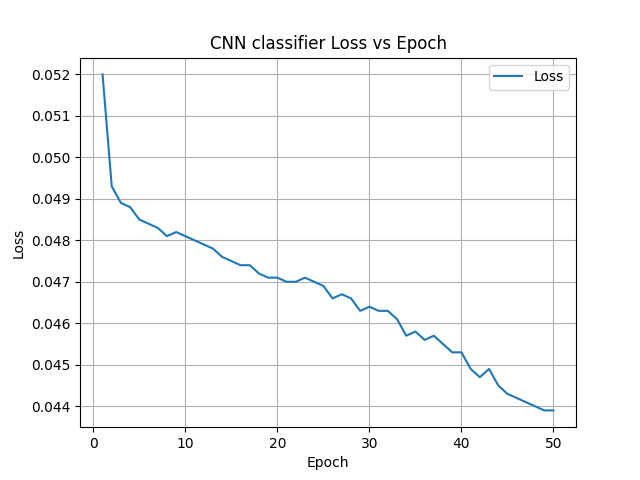
\includegraphics[width=4in]{image/loss_vs_epoch_train_log_2022-03-09_23-05-36}
        \caption{Loss Histogram of the CNN training}
        \label{fig:loss_hist}
    \end{figure}
    
    \par \hspace{15pt} Figure \ref{fig:loss_hist} shows the loss histogram of training the classifier model. According to the plot, the loss of the training is not plateaued at the ending training epoch, signifying that the model is still learning, yet at the end of 50 epochs, the model was able to give an output of around $80\%$ accuracy. Thus the group believe that with longer training time and better hardware accelerator, the model will be able to achieve better results. The group would try to investigate on further training with the next half of the project.

\end{par} %% Jerry
        % \subsubsection{subspace learning (vanilla version) result}
    \begin{par}
        \par \hspace{15pt} The team ran SVD on the pre-processd training dataset and plot the singular values. Figure \ref{fig:svd} shows the singular value plot for genre 3 as an example. Use these plots, the team obtained the orthonormal basis for all the genres. Then, all the testing data were projected to the orthogonal complement of these genre subspaces. In the end, the projected vectors were being compared and predictions were made. Unfortunately, using this method, a classification accuracy of only 10\% was achieved. One potential reason for this is insufficient amount of training data. Another potential reason for is music genres are too complicated to be classified by different subspaces.
    \end{par}
    
    \begin{par}
    \begin{figure}[H]
        \centering
        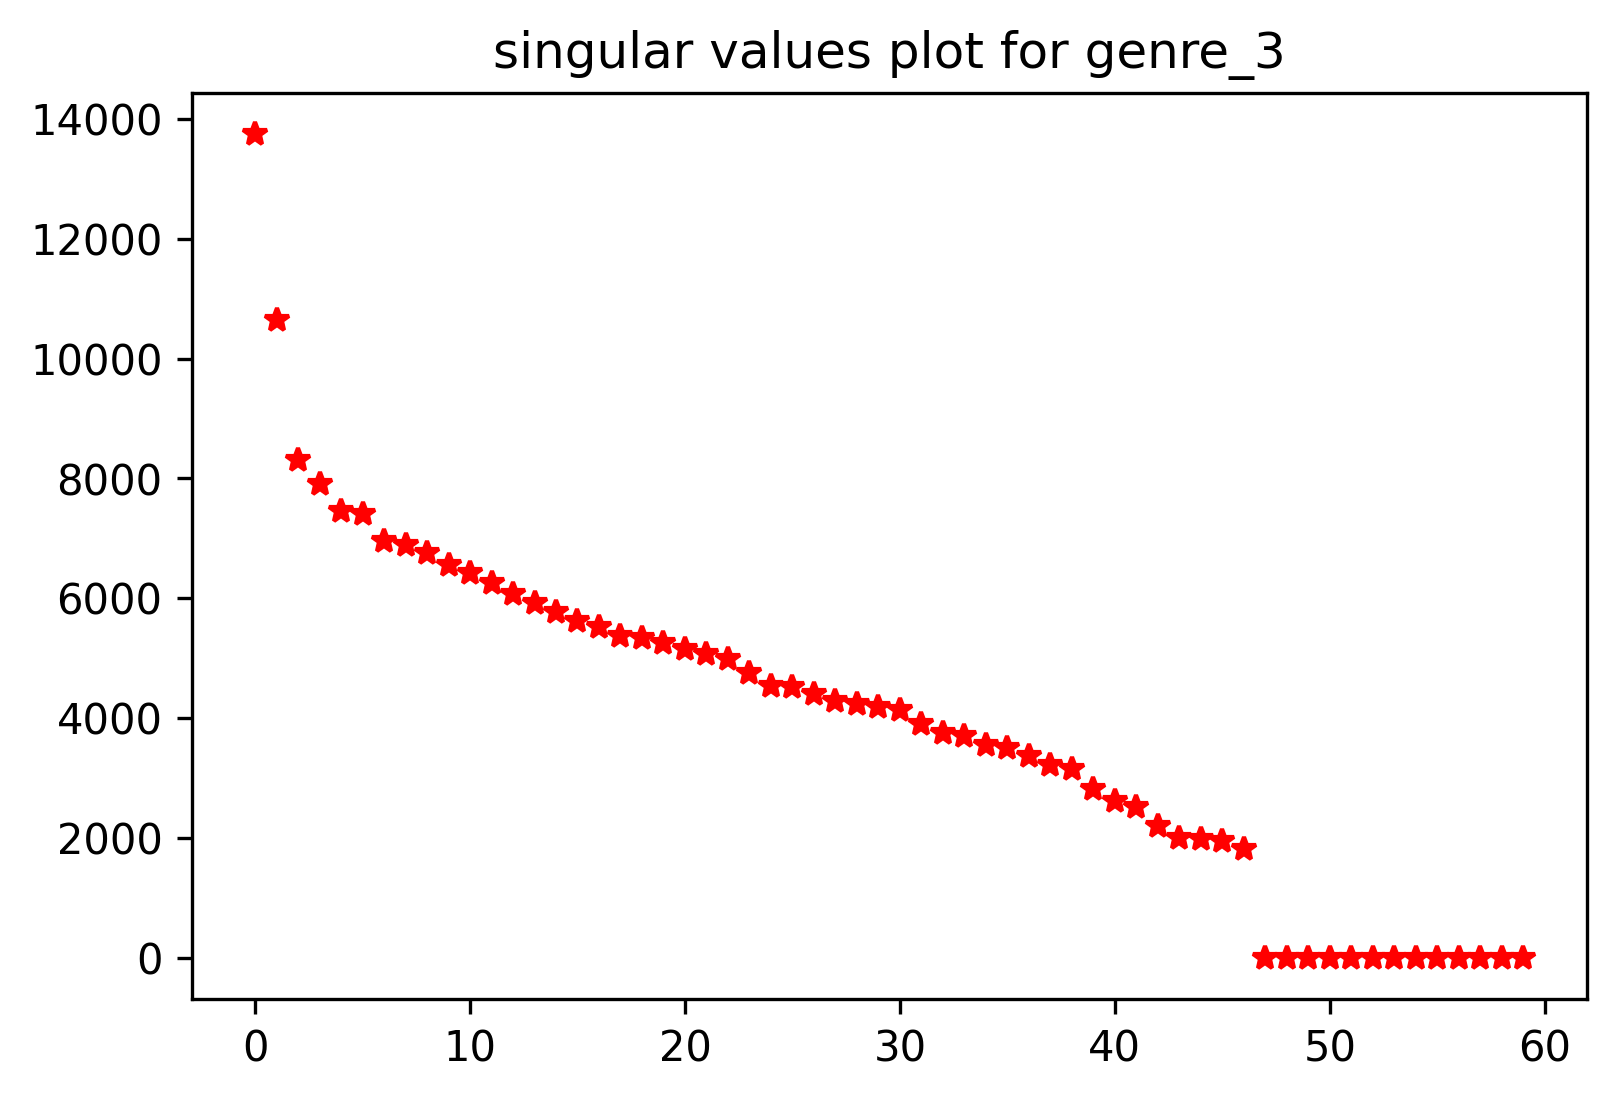
\includegraphics[width=4in]{image/s3_plot.png}
        \caption{Singular Value Plot for Genre 3}
        \label{fig:svd}
    \end{figure}
    \end{par} %% Congni
        % \begin{par}
    \subsubsection{Classification Result Using Mel-Frequency Cepstral Coefficient}
    \par \hspace{15pt} In order to retain an acceptable time-efficiency for the singular value decomposition required in the team's Sub-space Learning (SL) module, the team needs to shrink down the size of the song tracks. One challenge for this task is that the compression must make sure the prominent features of the song data stay distinguishable so an effective classification is possible. With this in mind, the team decides to adopt a feature extraction/representation method called Mel-Frequency Cepstral Coefficient (MFCC) in order to take out the most prominent patterns of the songs.
    \par MFCC is originally used to represent the power-spectrum of an acoustic signal. Since the coefficients of MFC are able to represent the frequency features (after applying Fourier transform) of the signal, this quantity is widely used in audio compression. Although the MFCC is originally designed to transform a time-amplitude signal, and that our data set are binary values, with pitch instead of amplitude of the sound recorded at each time-step, the team can still take advantage of its ability to describe the noticeable shape and patterns of a signal-the song tracks can be seen as time-amplitude signal where the amplitude equals, in numeric value, to the pitch at each time-step.
    \par The team tries to use the sets of MFCC for each song track instead of Pianoroll binary data before Mel-Frequency Cepstral transformation. The parameters used for calculating MFCC are the following: Sample-rate = 8000 Hz, Window length = 0.025, Window step = 0.01, Number of Cepstral Coefficient = 16, Number of Filters = 26. The sample-rate needs to be the power of 2, and it should reflect the frequency at which the sound signal is collected; the calculation of MFCC segments the sound signal into multiple pieces called "window", so the window length determines the length of each piece, while the window step determines the distance between two windows; therefore, decreasing window step increases the total number of MFCC calculated. Using MFCC as inputs to the subspace learning method, the team obtains a classification accuracy of 45 percent; a sample singular value plot is shown in Figure \ref{mfcc_svd} transforming the original data into MFCC matrices elevate the classification accuracy from 10 to 45 percent.

\end{par}
\begin{par}
    \begin{figure}[H]
        \centering
        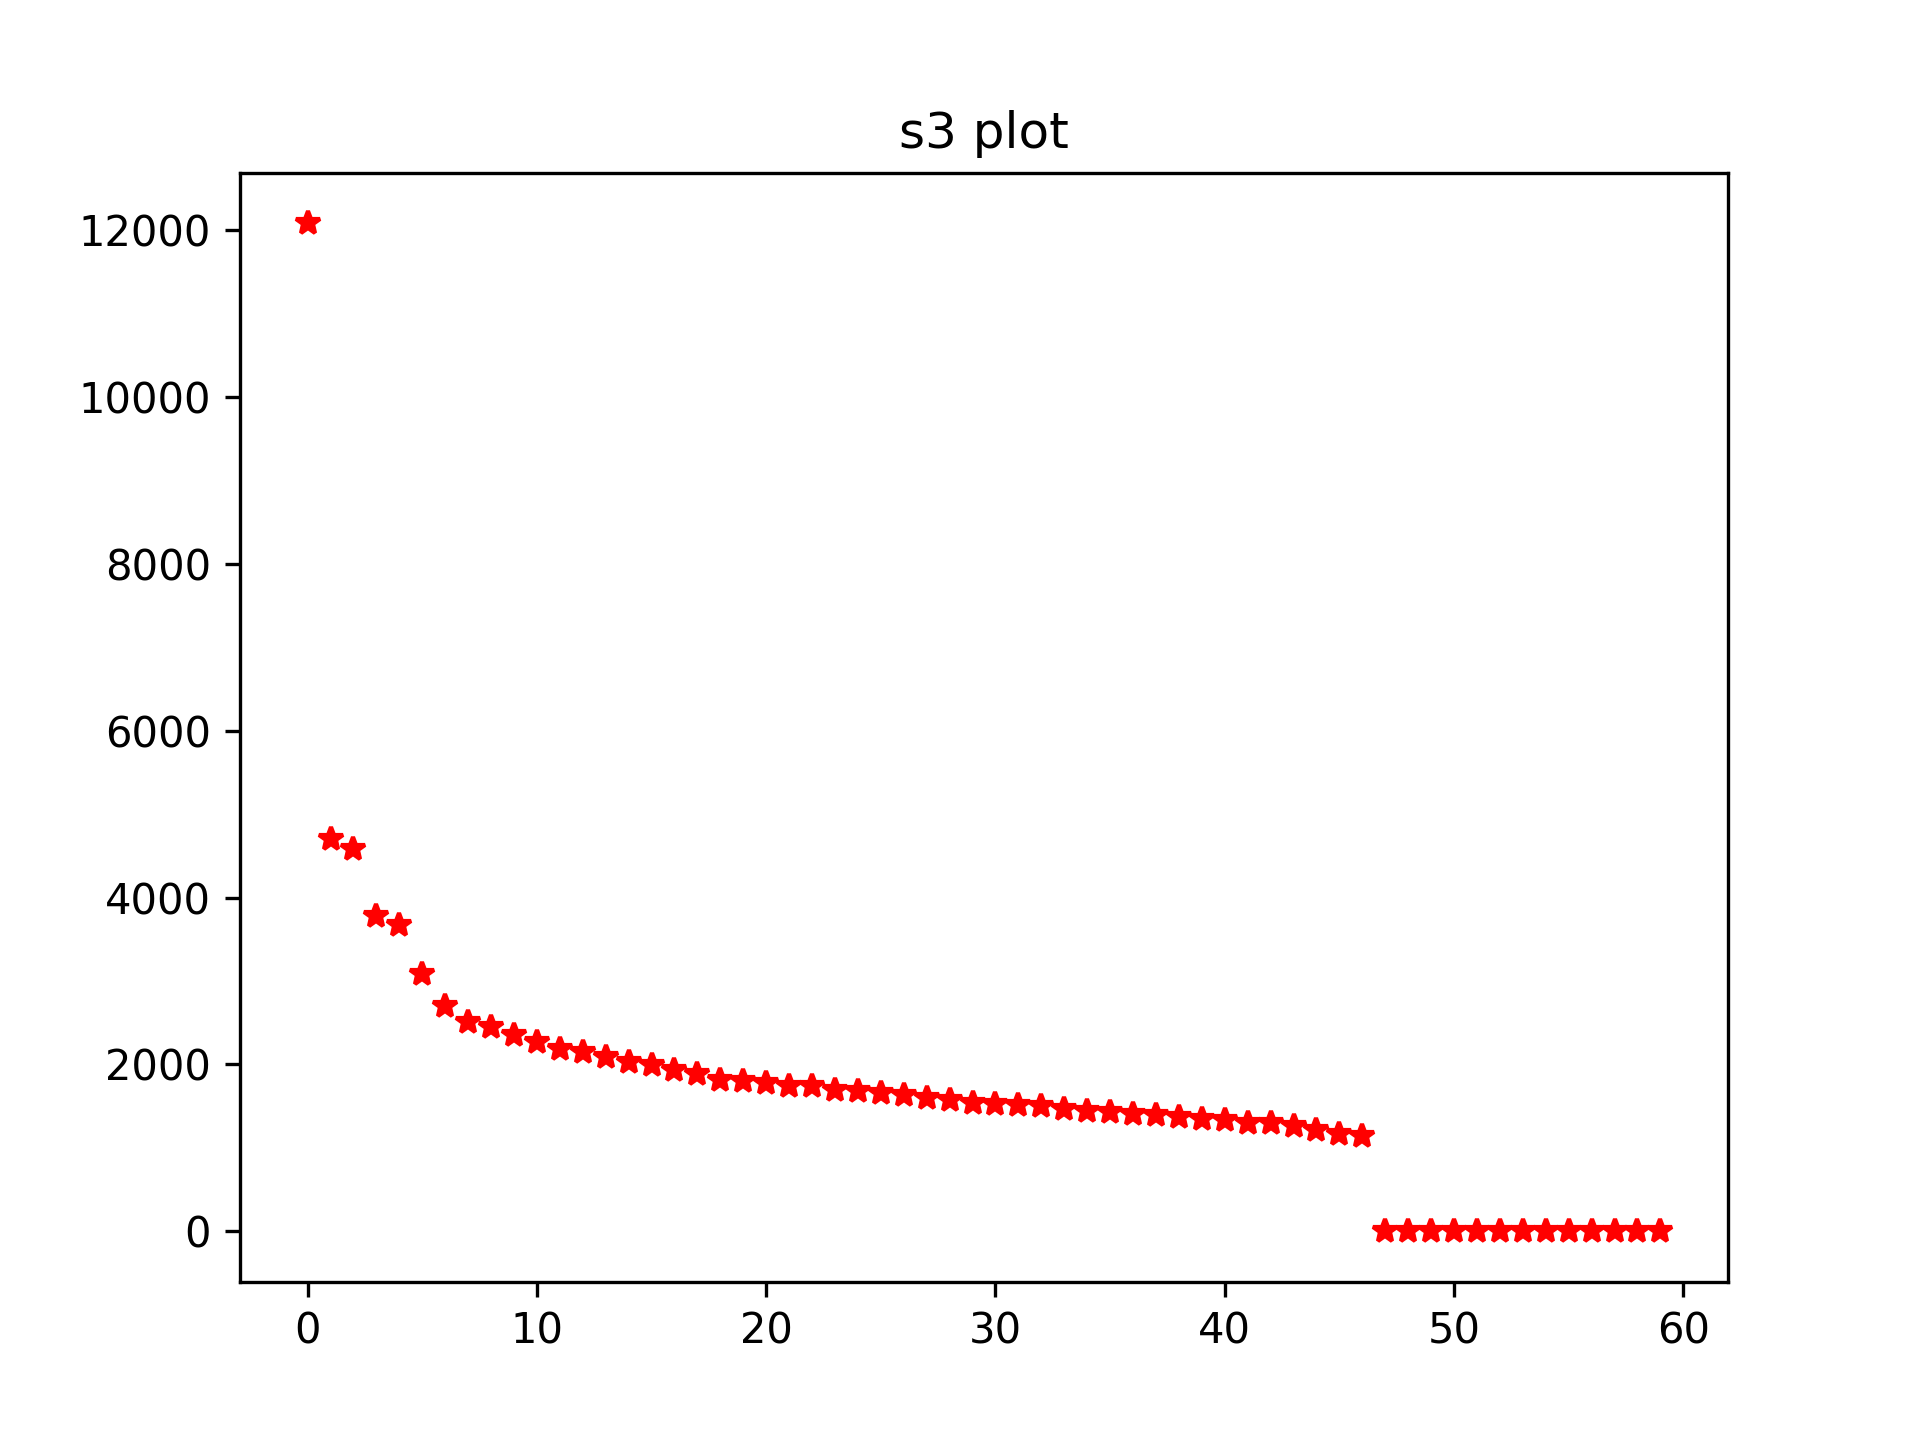
\includegraphics[width=4in]{image/s3_plot_mfcc.png}
        \caption{Singular Value Plot for Genre 3 (MFCC)}
        \label{fig:mfcc_svd}
    \end{figure}
    \end{par} %% Muye

    \subsection{Generator}
        \label{sub:exp_gen}
        % \input{experimental_generator} %% Muye

\section{Future Milestone}
    \label{sec:future}
    % \input{future} 
    %% for the next 6 weeks
    %% Dates and sub-goals
    %% Together

\section{Conclusion}
    \label{sec:conclusion}
    % \input{conclusion}

\section*{Author Contributions}
    \label{sec:contributions}
    % \begin{par}
    For this course project, Jerry Cheng has proposed the network architecture and their respective ablations, collected the data and constructed the customized dataloader. Jerry also finished the VGG-based CNN classifier. Congni Shi finished the naive SVD classifier, and incorporated the MFCC features once it was finished by Muye Jia. Muye wrote and tested the Generator and the MFCC feature extractor for the SVD classifier. Jerry oversees the cloud computing platforms and is in charge of the deployment of all deep learning models. All member contributed equally on this report. 
\end{par}

\bibliography{reference} % put your bibtex file here
\nocite{*}
\bibliographystyle{abbrv}


\end{document}

